\documentclass{sig-alternate}
\usepackage{enumitem}
\usepackage{multirow}
\usepackage{amsmath}
\usepackage{amssymb}
\usepackage{adjustbox}
\usepackage{float}
\usepackage{multirow}
\usepackage{xcolor}

\begin{document}

% CopyrightFXX
%\setcopyright{acmcopyright}
%\setcopyright{acmlicensed}
%\setcopyright{rightsretained}
%\setcopyright{usgov}
%\setcopyright{usgovmixed}
%\setcopyright{cagov}
%\setcopyright{cagovmixed}

\CopyrightYear{2016}
\setcopyright{acmcopyright}
\conferenceinfo{3rd International Digital Libraries for Musicology workshop (DLfM 2016)}{August 12 2016, New York, USA}
\isbn{978-1-4503-4751-8/16/08}\acmPrice{\$15.00}
\doi{http://dx.doi.org/10.1145/2970044.2970054}

%
% --- Author Metadata here ---
%\CopyrightYear{2007} % Allows default copyright year (20) to be over-ridden - IF NEED BE.
%\crdata{0-12345-67-8/90/01}  % Allows default copyright data (0-89791-88-6/97/05) to be over-ridden - IF NEED BE.
% --- End of Author Metadata ---

\title{MORTY: A Toolbox for \\Mode Recognition and Tonic Identification}

\numberofauthors{3}
\author{
% You can go ahead and credit any number of authors here,
% e.g. one 'row of three' or two rows (consisting of one row of three
% and a second row of one, two or three).
%
% The command \alignauthor (no curly braces needed) should
% precede each author name, affiliation/snail-mail address and
% e-mail address. Additionally, tag each line of
% affiliation/address with \affaddr, and tag the
% e-mail address with \email.
%
% 1st. author
\alignauthor
Altu\u{g} Karakurt\\
       \affaddr{The Ohio State University}\\
       \affaddr{Columbus, OH 43210}\\
       \email{karakurt.1@osu.edu}
% 2nd. author
\alignauthor
Sertan \c{S}ent\"{u}rk \\
       \affaddr{Universitat Pompeu Fabra}\\
       \affaddr{Roc Boronat, 138}\\
       \affaddr{Barcelona, Spain 08018}\\
       \email{sertan.senturk@upf.edu}
% 3rd. author
\alignauthor Xavier Serra\\
       \affaddr{Universitat Pompeu Fabra}\\
       \affaddr{Roc Boronat, 138}\\
       \affaddr{Barcelona, Spain 08018}\\
       \email{xavier.serra@upf.edu}
}
\date{submitted: 20 May 2016}

\maketitle
\begin{abstract}
In the general sense, mode defines the melodic framework and tonic acts as the reference tuning pitch for the melody in the performances of many music cultures. The mode and tonic information of the audio recordings is essential for many music information retrieval tasks such as automatic transcription, tuning analysis and music similarity. In this paper we present MORTY, an open source toolbox for mode recognition and tonic identification. The toolbox implements generalized variants of two state-of-the-art methods based on pitch distribution analysis. The algorithms are designed in a generic manner such that they can be easily optimized according to the culture-specific aspects of the studied music tradition. We test the generalized methodology systematically on the largest mode recognition dataset curated for Ottoman-Turkish makam music so far, which is composed of 1000 recordings in 50 modes. We obtained 95.8\%, 71.8\% and 63.6\% accuracy in tonic identification, mode recognition and joint mode and tonic estimation tasks, respectively. We additionally present recent experiments on Carnatic and Hindustani music in comparison with several methodologies recently proposed for raga/raag recognition. We prioritized the reproducibility of our work and provide all of our data, code and results publicly. Hence we hope that our toolbox would be used as a benchmark for future methodologies proposed for mode recognition and tonic identification, especially for music traditions in which these computational tasks have not been addressed yet.
\end{abstract}

\keywords{Mode recognition; Tonic Identification; Toolbox; Ottoman-Turkish makam music; Carnatic Music; Hindustani Music; Pitch Class Distribution; $k$-nearest neighbors classification; Open Source Software; Reproducibility}

\section{Introduction}\label{sec:introduction}
In many music cultures, the melodies adhere to a particular melodic framework, which specifies the melodic characteristics of the music. While the function and the understanding of these frameworks are distinct from a culture-specific perspective, in a broader sense they may be considered as the ``modes'' of the studied music culture. Some of the music traditions that can be considered as ``modal'' are Indian art musics, the makam traditions and medieval church chants~\cite{mode2016oxford}. Mode recognition is an important complementary task in computational musicology, music discovery, music similarity and recommendation. 

Tonic is another important musical concept. It acts as the reference frequency for the melodic progression in a performance. In many music cultures there is no standard reference tuning frequency, which makes it crucial to identify the tonic frequency to study melodic interactions. Estimating the tonic of a recording is the first step for various computational tasks such as tuning analysis~\cite{tuning}, automatic transcription~\cite{transcription} and melodic motif discovery~\cite{gulati_network}.

There has been a extensive interest on mode recognition in the last decade~\cite{koduri2012ragaReview}. Most of these work focus on culture-specific approaches for music traditions like Otto\-man-Turkish Makam music (OTMM)~\cite{bozkurt_makam}, Carnatic music~\cite{dighe, dighe2, gulati_network}, Hindustani music~\cite{chordia2, chordia,gulati2016raga} and Dastgah music~\cite{dastgah}. A considerable portion of these studies are based on comparing pitch distributions~\cite{chordia2, chordia, dighe, dighe2, bozkurt_makam}, which are shown to be reliable in the mode recognition task. There also exists recent approaches that are based on characteristic melodic motif mining using network analysis~\cite{gulati2016raga,gulati_network}, aggregating note models using automatic transcription~\cite{koduri2014intonation} or audio-score alignment~\cite{senturk2016noteModel_smc} and classification using neural networks~\cite{raga_mining, neural_raga_chapter}, all of which are designed specific to the studied music culture and are not generalizable to other music cultures without considerable effort. Similarly, several studies on tonic identification use pitch distribution based methods~\cite{bozkurt_tonic, chordia}. More recently there has been an interest in culture specific methods for this task~\cite{sercan_tonic, sankalp_tonic, senturk2013karar_ismir} that make use of heuristics and the musical characteristics of the studied tradition. 

In these studies, the features extracted from the data,\footnote{Excluding the commercial audio recordings, which cannot be generally made public due to copyright laws.} source code and the experimental results are not usually shared. We consider the unavailability of public tools, data\-sets and reproducible experimentations as major obstacles for computational music information research, especially if the relevant tasks have not been applied to studied music traditions earlier.

We present MORTY (\textbf{MO}de~\textbf{R}ecognition and~\textbf{T}onic \textbf{Y}den\-tification Toolbox), an open source toolbox written in \emph{Python} for mode recognition and tonic identification. It contains a generalized implementation of two pitch distribution based methods proposed for Ottoman-Turkish makam music~\cite{bozkurt_tonic, bozkurt_makam} and Hindustani music~\cite{chordia}. Our primary aim is to provide open and flexible tools for the mode recognition and tonic identification tasks, which can be applied to different music cultures while allowing the users to optimize the parameters easily according to the characteristics of the studied music. MORTY may be (and has been, see Section~\ref{sec:hindustani_carnatic}) used as a benchmark against novel methodologies proposed. 

Another motivation for this work is to provide tools for several relevant tasks such as tuning and intonation analysis~\cite{bozkurt_makam}. Combined with automatic tonic identification and makam recognition, these features would facilitate the curation and description of large audio corpora not only by greatly reducing the time and effort spent on manual annotations but also providing automatically extracted, reliable information, which would be too difficult or time-consuming for human annotators.

Our contributions can be summarized as:
\begin{enumerate}[noitemsep]
\item An open toolbox aimed to set a benchmark for future research in mode recognition and tonic identification, which implements and generalizes the state of the art methodologies proposed by Bozkurt and Gedik~\cite{bozkurt_tonic, bozkurt_makam}, and Chordia and \c{S}ent\"{u}rk~\cite{chordia}
\item The largest makam recognition dataset for Ottoman-Turkish Makam Music (OTMM), composed of 1000 audio recordings from 20 makams with annotated tonic frequency and editorial metadata.
\item Exhaustive and reproducible evaluation of the aforementioned two state of the art methods on the Otto\-man-Turkish makam recognition dataset.
\item Improving the state of the art in tonic identification met\-hod applied to OTMM
\item Mode recognition experiments on Hindustani and Carnatic music traditions to demonstrate the applicability of our implementations on different music cultures.
\end{enumerate}

The rest of this paper is organized as the following: Section~\ref{sec:problem} provides formal definitions of the problems. Section~\ref{sec:morty} presents the implementation details and the features of our toolbox. Section~\ref{sec:methodology} describes the two state of the art methods and their implementations in detail. Section~\ref{sec:experiments} explains the experiments and the obtained results on our OTMM dataset and Section~\ref{sec:hindustani_carnatic} presents our results on Carnatic and Hindustani cultures. Finally, we discuss the results we obtained in Section~\ref{sec:discussion} and conclude with our comments and suggestions for the future work in Section~\ref{sec:conclusion}.

For the sake of open research and reproducability, the toolbox (Section~\ref{sec:morty}) the dataset (Section~\ref{sec:dataset}), experiments (Section~\ref{sec:experiments}) and results (Section~\ref{sec:results}) are accesible publicly via CompMusic website.\footnote{http://compmusic.upf.edu/node/319}

\section{Problem Definition}\label{sec:problem}
We define \emph{mode recognition} as classifying the mode $\zeta^{(a)}$ of an audio excerpt $(a)$ from a discrete set of modes $Z := \{\zeta_1, \dots, \zeta_V\}$, where $\zeta^{(a)} \in Z$ and $V$ is the total number of modes. The mode set is specific to music culture being studied. In mode recognition, we assume that the tonic frequency $r^{(a)}$ of the audio recording is available.

We define \emph{tonic identification} as estimating the frequency or the pitch class (if the octave information of the tonic is not well-defined for the music culture or the performance) of the performance tonic. We denote the tonic of an audio excerpt as $r^{(a)}$. Unlike mode, tonic is a continuous variable. However, in practice, the tonic is typically constrained to be one of the stable pitches or pitch classes performed in the audio excerpt~\cite{chordia,bozkurt_makam}. With this assumption, tonic identification can be reformulated as estimating the tonic frequency or the pitch class $r^{(a)}$ from a finite set of stable frequencies/pitch-classes $R := \{r_1, \dots, r_W^{(a)}\}$ performed in an audio excerpt $(a)$, where $r^{(a)} \in R$ and $W^{(a)}$ is the number of the stable pitches in the audio excerpt. In tonic identification, we assume that the mode $\zeta^{(a)}$ of the recording is known. 

A third scenario arises when both the tonic $r^{(a)}$ and the mode $\zeta^{(a)}$ of the recording $(a)$ are unknown. In this case, we identify the tonic and recognize the mode together, which we term as \emph{joint estimation}.

Note that these scenarios are actually multi-class problems, since the mode and the tonic may change throughout the performance. This is a more challenging problem, where we would not only like to obtain the set of the modes and tonics in the performance but also mark the intervals, where these musical ``attributes'' are observed.\footnote{A manually annotated example for OTMM is given in \url{http://musicbrainz.org/recording/37dd6a6a-4c19-4a86-886a-882840d59518}} There has not been any generalizable method proposed for either mode recognition or tonic identification in such a scenario yet. In MORTY, we restrict the problem on mode recognition and tonic identification of audio excerpts with a single mode and tonic, and leave the multiple estimation problem as a future work to investigate.

\section{MORTY}\label{sec:morty}

MORTY (\textbf{MO}de~\textbf{R}ecognition and~\textbf{T}onic~\textbf{Y}dentification Toolbox) is free software, licensed under \emph{Affero GPLv3}.\footnote{\url{https://github.com/altugkarakurt/morty}} It is implemented in \emph{Python $2.7$} and uses the open source \emph{NumPy} and \emph{SciPy} libraries for numeric computations, \emph{scikit-learn} for machine learning related tasks and \emph{Essentia}~\cite{bogdanov2013essentia} for audio processing. Since our motivation is handling large audio collections like digital libraries, we also provide parallelization through \emph{ipyparallel}, a part of \emph{Jupyter} project\footnote{\url{https://jupyter.org/}}.

As a user manual, we provide \emph{Jupyter} notebooks that demonstrate example usage for each method (Section~\ref{sec:methodology}), as well as examples for parallelization.\footnote{\url{https://github.com/altugkarakurt/morty/blob/e927386dc72e6282f0ccfaf1c390625f2a554268/demos/knn_demo.ipynb}} The toolbox was implemented with a modular approach such that it is easy to modify and extend, which makes it possible for future users to contribute with new features, as well as to customize the implementations according to their needs.

\section{Methodology}\label{sec:methodology}

In MORTY we combine and generalize the two state of the art methods, originally proposed for audio recordings of OTMM~\cite{bozkurt_tonic,bozkurt_makam} and short audio excerpts of Hindustani music~\cite{chordia}. The generalized methods are supervised and use $k$-nearest neighbors ($k$-NN) estimation for classification. Our implementations are generic such that the parameters selected in the feature extraction, training and testing steps can be optimized for the properties of the studied music tradition. We also allow the user to classify either short audio excerpts or complete audio recordings and switch between different features, training schemes and tasks as introduced in~\cite{bozkurt_tonic, chordia, bozkurt_makam}. %Later in Section~\ref{sec:experiments}, we demonstrate the experiments for the parameter selection and optimization on a test dataset of OTMM (Section~\ref{sec:dataset}) and in Section~\ref{sec:hindustani_carnatic} the reproduced results of~\cite{chordia} on a Hindustani and a Carnatic music dataset using the optimal parameters reported in~\cite{chordia}.

In the training step we use audio excerpts with annotated mode and tonic. We first extract a predominant me\-lody for each audio excerpt. These are used to compute either pitch distributions (PD) or pitch class distributions (PCD) (Section~\ref{sec:feature}). Next, we create mode models from these computed distributions (Section~\ref{sec:training}). 

Given an audio recording with an unknown mode and/or tonic, we extract its predominant melody and compute the distribution. Then, we compute a distance or dissimilarity between the distribution of the test audio and the selected distributions in the training models and compute the $k$ nearest neighbors according to the computed measure (Section~\ref{sec:distance}). Finally, we estimate the unknown mode and/or tonic as the most common candidate among the $k$ nearest neighbors (Section~\ref{sec:mode}-\ref{sec:joint}).

Now we proceed to explain the generalized methodology in detail. We label the tasks, features, training models and parameters in MORTY explicitly with the letters {\bf T, F, M} and {\bf P} throughout this Section for the sake of clarity.

\subsection{Feature Extraction}\label{sec:feature}
The first step of method is predominant melody extraction {\bf(F1)}~\cite{bozkurt_tonic, chordia, bozkurt_makam}. As discussed in~\cite{atli2014makamFeature_atmm} and~\cite{bozkurt_tonic}, the quality of the extracted pitch predominant melody directly affects the reliability of the computed models and predominant melody extraction methods optimized or designed for the culture-specific aspects of the studied music might be desirable at this step. The implementation of such an algorithm is outside the scope of MORTY. 

We denote the predominant melody extracted from an audio excerpt, $(a)$, as $X^{(a)}  \triangleq \left(x^{(a)}_1 \dots x^{(a)}_I\right)$, where $x^{(a)}_i \in  X^{(a)}$ is a pitch sample and $i \in [1: I]$, where $I$ is the length of the predominant melody. 

Next, the samples in the predominant melody are converted to the cent scale using the equation below:

\begin{equation}
\label{eq:cent_norm}
x^{(r)}  \triangleq 1200 \log_2\left(\frac{x}{r}\right)
\end{equation}

Here, $x^{(r)}$ denotes the cent distance of the frequency $x$ from the reference frequency $r$. In the training step (Section~\ref{sec:training}) and the mode recognition task (Section~\ref{sec:mode}), i.e. when the annotated tonic is available, $r$ is the annotated tonic frequency of the audio excerpt. In the tonic identification and joint identification tasks the predominant melody will be normalized with respect to the several tonic candidates one by one, one of which will be identified as the tonic (Section~\ref{sec:tonic}).

Using the normalized predominant samples we compute either a pitch distribution (PD) as used in~\cite{bozkurt_makam} or a pitch class distribution (PCD) as used in~\cite{chordia}. PD and PCD shows the relative occurrence of the pitch and pitch class values with respect to each other, respectively. Throughout the text we simply refer the PDs and PCDs collectively as ``distributions'' {\bf (F2)}. The values in both distributions are computed as:

\begin{equation}
	h_n  \triangleq \frac{\sum_{i=1}^I \lambda_n\left(x_i\right)}{I}
	\label{eqn:histogram}
\end{equation}

\noindent
where $h_{n}$ is the occurence computed for the $n$-th bin in the distribution $h$, computed samples $x_i \in X$ in the normalized pitch and $I$ is the number of pitch samples.

The accumulator function $\lambda$ for PDs is defined as:

\begin{equation}
\lambda_{n}(x) \triangleq
\begin{cases}
1, & c_{n} \leq x \leq  c_{n+1} \\
0, & \text{otherwise} \\
\end{cases}
\end{equation}

\noindent
where $x$ is a normalized pitch sample and $(c_{n}, c_{n+1})$ are the boundaries of the $n$-th bin. 
Similarly the $\lambda$ function for PCDs is defined as:
\begin{equation}
\lambda_{m}(x)  \triangleq
\begin{cases}
1, & c_{n} \leq \left(x\,\bmod\,1200\right) \leq  c_{n+1} \\
0, & \text{otherwise} \\
\end{cases}
\end{equation}

Note that the PCD is a ``circular'' feature, e.g. the first and the last bins are next to each other. Also notice that both PD and PCD are normalized such that the resultant distribution can be treated as a probability density function. 

The bin size $\beta$ {\bf (P1)} of the distribution determines how precise the distribution is (to the extend allowed by the cent-precision of the predominant melody) in representing the pitch space, the tuning of the stable pitches and the microtonal characteristics in a lower-level. The computed distributions might need to have a small bin size, e.g. less than a quarter tone ($50$ cents) for many music cultures~\cite{chordia,bozkurt_makam}. We select a constant bin size for the computed distributions, i.e. $\beta = c_{n+1} - c_{n},  \forall n$. The bin centers of both PDs and PCDs are selected such that the reference frequency $r$ is represented as a bin centered around $0$ cents. We denote the number of bins in a distribution as $N$. Note that $N$ equals to $\lfloor1200 / \beta\rfloor$ in a PCD.

To remove the spurious peaks in the distribution we convolve it with a Gaussian kernel and obtain a ``smoothed'' distribution~\cite{chordia}. The standard deviation of the Gaussian kernel, termed as the kernel width $\sigma$ {\bf (P2)}, determines how smooth the resulting distribution will get. The kernel width should be comparable to the bin size {\bf (P1)} since a value lower than one third of the bin size would not contribute much to smoothing\footnote{The values of the bins in a Gaussian kernel, which are more than three standard deviations away from the mean are greatly diminished.} and a high value would ``blur''  the distribution too much. Moreover, this parameter has a direct impact on the number and the location of tonic candidates in tonic identification (Section~\ref{sec:tonic}), which might effect both the accuracy and the processing time. In our implementation, we select the overall width of the Gaussian kernel as 5 times the kernel width from peak to tail for performance reasons.

\subsection{Training Model}\label{sec:training}
As mentioned earlier, the implemented method is supervised and hence require training data, i.e. audio excerpts with the annotated mode and tonic. From a training audio excerpt $(a)$, we first extract the predominant me\-lody $X^{(a)}$ and normalize with respect to the annotated tonic frequency $r^{(a)}$ (Equation~\ref{eq:cent_norm}). Next, the normalized predominant melo\-dies $X^{\left(a, r^{(a)}\right)}$ are grouped according to the annotated mode $\zeta^{(a)}$ of each individual excerpt. 

\begin{figure}
\centering
\includegraphics[width=.8\columnwidth]{figures/bozkurt_pcd}
\caption{An example model with single PCD per mode trained for three OTMM makams}
\label{fig:bozkurt_training}
\end{figure}

\begin{figure}
\centering
\includegraphics[width=.8\columnwidth]{figures/chordia_pcd}
\caption{An example model with three PCDs per mode trained for three OTMM makams}
\label{fig:chordia_training}
\end{figure}

The fundamental difference between the methods proposed in~\cite{chordia} and~\cite{bozkurt_makam} is the training model {\bf (M)} obtained in the training step. The methodology proposed in~\cite{bozkurt_tonic, bozkurt_makam} joins all the normalized predominant melodies and compute a single distribution per mode. On the other hand,~\cite{chordia} creates a separate distribution from each annotated excerpt $(a)$. From a machine learning perspective~\cite{bozkurt_makam} represents each mode with a single data point (Figure~\ref{fig:bozkurt_training}), whereas~\cite{chordia} represents them with many (Figure~\ref{fig:chordia_training}) in an $N$-dimensional space, where $N$ is the number of bins in the distributions. From now on, we term the training models using the training step in~\cite{bozkurt_tonic, bozkurt_makam} and~\cite{chordia} as ``single distribution per mode'' and ``multi-distributions per mode'', respectively. We denote the obtained model as $M \triangleq \{m_1, m_2, \dots\}$. $m_j \in M$ is a tuple $\langle h_j, \zeta_j\rangle$, where $h_j$ and $\zeta_j$ denotes the trained distribution and the mode label of $m_j$, respectively. The model $M$ consists of the distribution representations for $V$ modes, where $V$ is the number of unique mode labels $\zeta_v, v \in \{1,..,V\}$ in the training excerpts.

\subsection{Nearest Neighbor Selection}\label{sec:distance}
In mode recognition, tonic identification and joint estimation tasks (Section~\ref{sec:mode}-\ref{sec:joint}), the common step is to find the nearest neighbor(s) of a selected distribution among a set of distributions to be compared against. To find the nearest neighbors we compute a distance or a dissimilarity between the test distribution and each distribution in the comparison set~\cite{distance}. We have currently implemented the distance and the similarity metrics in~\cite{bozkurt_makam, chordia}, namely, City-Block ($L_1$ Norm) distance, Euclidean ($L_2$ Norm) distance, $L_3$ Norm, Bhattacharyya distance, intersection and cross correlation {\bf (P3)}. Note that intersection and cross correlation are similarity metrics, hence we convert them to dissimilarities (i.e. $1 - $similarity) instead. The choice of the distance or dissimilarity measure plays a crucial role in the neighbor selection.

After the distances or the dissimilarities are computed, the compared distributions are ranked and the $k$ {\bf (P4)} nearest neighbors are selected. We then estimate the test sample as the most common label of the neighbors. In case of a tie between two or more groups, we select label of the group, which accumulates the lowest distance or dissimilarity. Note that if a single-distribution is computed for each mode ({\bf M} as explained in Section~\ref{sec:training}), the $k$ value is always 1, since each mode is only represented by one sample.

Now we proceed to explain the procedure for each task {\bf(T)} in detail.

%The implemented metrics are given below:
%
%\begin{itemize}[noitemsep]
%\item City-Block ($L_1$ Norm) Distance:
%\begin{equation}
%\frac{1}{M}\sum\limits_{m=1}^{M}|h^{(r)}_m - h^{(t)}_m|
%\end{equation}
%
%\item Euclidean ($L_2$ Norm) Distance:
%\begin{equation}
%\sqrt{\sum\limits_{m=1}^{M}\left(h^{(r)}_m - h^{(t)}_m\right)^2}
%\end{equation}
%
%\item $L_3$ Norm:
%\begin{equation}
%\left(\sum\limits_{m=1}^{M}|h^{(r)}_m - h^{(t)}_m|^3\right)^{1/3}
%\end{equation}
%
%\item Bhattacharyya Distance:
%\begin{equation}
%-\log\sum\limits_{m=1}^{M}\sqrt{h^{(r)}_mh^{(t)}_m}
%\end{equation}
%
%%\item Jensen-Shannon Distance:
%%\begin{equation}
%%\sum\limits_{m=1}^{M}XX
%%\end{equation}
%%
%%\item Jeffrey's Divergence:
%%\begin{equation}
%%\sum\limits_{m=1}^{M}XX
%%\end{equation}
%
%\item Inverse of Intersection:
%\begin{equation}
%\left(\frac{1}{M}\sum\limits_{m=1}^{M}min\left(h^{(r)}_m, h^{(t)}_m\right)\right)^{-1}
%\end{equation}
%
%\item Negative of Cross-Correlation:
%\begin{equation}
%1 - \frac{1}{M}\sum\limits_{m=1}^{M}h^{(r)}_m h^{(t)}_m
%\end{equation}
%\end{itemize}
%
%\noindent
%where $h^{(r)}_m$

\subsection{Mode Recognition}\label{sec:mode}
Given an audio excerpt $(b)$ with an unknown mode, we compute the distribution $h^{\left(b, r^{(b)}\right)}$ by taking the annotated tonic $r^{(b)}$ as the reference (Section~\ref{sec:feature}). Next we compute the distance or the dissimilarity between $h^{\left(b, r^{(b)}\right)}$ and the trained distribution $h_j$ of each $m_j$, $\forall m_j \in M$, where $M$ is the trained model, and obtain the $k$ nearest neighbors to $(b)$. We estimate the mode of $(b)$ as the most common label $\zeta_v$ within the nearest neighbors as explained in Section~\ref{sec:distance}.

\subsection{Tonic Identification}\label{sec:tonic}

Given an audio excerpt $(b)$ with the annotated mode $\zeta^{(b)}$, we first extract the predominant melody $X^{b}$. Then we compute a distribution $h^{(b, *)}$ by taking an arbitrary frequency $(*)$ as the reference frequency (Section~\ref{sec:feature}). We detect the peaks in the distribution using the method explained in~\cite{smith1987parshl}. The peaks indicate the stable pitches performed in the excerpt. We only consider the peaks, which have a ratio between its height and the maxima of the distribution above a constant threshold {\bf (P5)}. We denote the set of tonic candidates as $R \triangleq \{r_1, \dots, r_{W^{(b)}}\}$, where $W^{(b)}$ is the number of detected peaks. The cent distance between $r_w$ and $*$ (Equation~\ref{eq:cent_norm}) is given as $r_w^{(*)} := \left(n_w - n_*\right) \times \beta,\,\forall l \in W^{(b)}$, where $\beta$ denotes the bin size {\bf (P1)} of the distribution {\bf (F2)}, and $n_w$ and $n_*$ are the bin indices, in which $l$ and $*$ reside in, i.e. $\lambda_{n_{l}}(l) = \lambda_{n_{*}}(*) = 1$ (Equation~\ref{eqn:histogram}). Assuming each of the peaks $r_w$ as the tonic candidate, we shift the distribution $h^{(b, *)}$ and obtain $h^{(b, r_w)}$ such that the $n$-th bin becomes the $(n + n_* - n_w)$-th for the PDs and the $(n + n_* - n_w \, mod \, N)$-th (where $N$ is the total number of bins) for the PCDs, respectively and the $n_w$-{th} bin represents $0$ cents in the shifted distribution.

From the training model M, we select all the $m_j$ $\in M$ with the label $\zeta^{(b)}$. Next we compute the distance or the dissimilarity between each shifted distribution $h^{(b, r_w)}$ and the selected $m_j$s. We select the $k$ pairs with the lowest distance or dissimilarity and select the most occurring peak $r_w$ in the neighbors as the estimated tonic (Section~\ref{sec:distance}).

\subsection{Joint Estimation}\label{sec:joint}
Given an audio excerpt $(b)$ with unknown mode and tonic, we compute the tonic candidates, $R \triangleq \{r_1, \dots, r_{W^{(b)}}\}$ and the distributions $h^{(b, r_w)}$ assuming each $r_w \in R$ as the tonic candidate as explained in Section~\ref{sec:tonic}. Next we compute the distance or the dissimilarity between each pair of shifted distribution $h^{(b, r_w)}$ and $m_j$ $\in M$. We select the $k$ pairs with the lowest distance or dissimilarity and estimate the most occurring $\langle$mode, tonic candidate$\rangle$ pair, i.e.  $\langle \zeta_v, r_w \rangle$ as the mode and the tonic (Section~\ref{sec:distance}).

%For these estimation problems, one of the distinguishing features of a recording is the occurrence frequencies of pitches cite, which is called the recording's \textit{pitch distribution} or \textit{PD}. It is computed by extracting the predominant melody of the recording and computing its normalized histogram. We discretize the frequencies, by defining a bin size. We map the frequencies within this range to the same bin. This range should be narrow enough to be informative and wide enough to prevent redundancy, hence it is our first parameter to be tuned.
%
%Even the optimally discretized PDs still have redundancy in them. For our purposes, some frequencies contribute to neither discrimination of modes nor identification of stable pitches. These frequencies appear due to various musical events like vibratos and slides, as well as factors like timbre and dynamics of instruments used, which are out of this work's scope. Following this observation, we consider a more compact and higher level derivative of this feature. \textit{Pitch class distribution} or \textit{PCD} is the octave wrapped version of PD. In other words, unlike PD, PCD exploits the octave information to map the occurrences of different frequencies of the same pitch class to the same value. For example, while PD represents 110 Hz, 220 Hz and 440 Hz as independent frequencies, PCD is informed about the harmonic relationship between these and maps them to the same bin. Hence, PCD provides a more compact representation for distribution of pitches. Clearly, the octave information is lost in this step, but since we are possibly dealing with heterophonic recordings of instruments which don't necessarily have the same spectral ranges, the lost information isn't really informative, but acts as noise for our purposes. Note that if PCD is used as the feature in the tonic identification process, we find the tonic pitch class, the octave is sometimes ambiguous in different cultures, but there are straightforward culture-specific methods~\cite{sercan_tonic,sankalp_tonic}
%
%These two features collectively are referred to as \textit{pitch histograms}. It is possible to smoothen pitch histograms by using methods like kernel density estimation~\cite{chordia} or moving averaging~\cite{bozkurt_tonic} before normalizing them. This process combines the local adjacent peaks and reduces the number of peaks by filtering out the spurious neighbor peaks around the stable pitches. In our implementations, we are using a Gaussian kernel for this procedure. It is possible to improve the algorithms' efficiency with this step, since the number of peaks of a pitch histogram substantially influences the computational cost of processing it, as peaks are treated as the set of tonic candidates. 
%
%As mentioned in Section 1, the tonic information allows us to computationally compare recordings uniformly. The way to do so is to represent the frequencies in the predominant melody with respect to their distance from a reference frequency. If the tonic is known it is treated as the reference point, but during the tonic estimation process, we use a dummy reference frequency since tonic is unknown. The unit that gives us this opportunity is cent. The conversion of a frequency value in Hz units to cents can be done using the following equation.

%Since our goal is to obtain culture-independent tools, we make the bin size parameter variable as mentioned in Section 4. In applications specific to modal music domain, there are many state of the art algorithms based on pitch histograms, such as ...(makam, raga, raag) cite. This demonstrates the representative nature of this feature when it comes to recordings of modal music traditions. Moreover, pitch histograms are computationally very convenient. They allow us to represent recordings with a vector of much smaller size compared to sparser alternatives such as the predominant melody or spectrogram of the recording. This shrinkage in data to be processed, impacts the performance of the methods, which would be crucial for real-time applications and big data tasks, such as analyzing entire digital libraries or corpora.

 
%\section{Single Histogram Mode Models}
%Single histogram mode models was proposed as a method specific to OTMM culture, by Gedik \& Bozkurt for tonic identification~\cite{bozkurt_tonic} and makam~\cite{bozkurt_makam} recognition. This approach is based on computing pitch histograms for modeling each mode and using these as the data points for representing the corresponding makams. Then, depending on the problem it uses the distance of the input recording's histogram with makam models in the prediction step. The paper does not report experiments on the joint estimation problem and assumes that one of the two parameters is known beforehand.
%
%First step of building a makam model is to extract the predominant melodies of the recordings that belong to that class. Then, the frequency values in these vectors are converted to cents and joined together to form a long predominant melody vector in cents. The pitch histogram of which is computed and used as the feature to represent the makam. Computationally, this is a very efficient approach, since each makam is represented by a single pitch histogram. The training process of this method consists of these steps and is completed when the pitch histogram representations of all makams are computed.
%
%For makam recognition, the computed makam models are loaded and the pitch distribution of the input recording is computed using the same parameters as in the training phase. Then, the input pitch histogram is compared using a chosen distance formulation. The makam estimate of the method is the one whose pitch histogram has the smallest distance from the input recording's.
%
%For tonic identification, the pitch histogram is computed using a dummy reference frequency and the peaks in this representation are detected. Then, the histogram is compared with the histogram of its known makam by treating each of these peaks as candidate tonics and shifting them to 0 cent frequency. Whichever peak gives the smallest distance is the predicted tonic frequency of the recording.
%
%When we analyzed this approach, we saw some room for improvement and introduced some extensions. As the pitch histogram representation, Bozkurt only uses PD. We included PCD in our implementations, which substantially improved the accuracy of this method in each of the three problems. We added $L_3$ norm to the set of candidate distances.
%
%In order to fully span our framework, we extended this approach to joint estimation problem. In that scenario, the distances are calculated for each peak frequency and mode combination and the pair which has the smallest distance is chosen as the predicted mode and tonic.
%
%\section{Multi-Histogram Representation of Modes}
%The other method we consider is proposed by Chordia \& Şentürk for joint estimation problem~\cite{chordia}. This method was proposed for joint tonic and raag recognition for Hindustani music culture, which we again extend to a general purpose framework for any modal music culture under inspection. 
%
%Unlike histogram mode models approach, this method treats each training sample's pitch histogram as a labeled data point in the feature space. So, the raags are represented with as many points as the available number of recordings in the training dataset. Other than this different perspective of representation, this method is very similar to single-histogram mode model approach~\cite{bozkurt_makam,bozkurt_tonic}. As a demonstration of this representation, Figure 3 shows five three chosen recordings per three makams from our dataset. With this representation, it is possible to capture the nuances within a mode by storing numerous performances that introduce slight variations from it.
%
%The training phase consists of pitch histogram generation of recordings. However, the estimation phase is different due to the multi-point representation. For joint estimation, we consider the \textit{k} many peak and mode pairs that give rise to the smallest distances and the prediction for each is determined by the majority vote among these. In case of a tie, we pick the one with the closest data-point to the input recording's histogram. Hence, we introduce \textit{k} as another adjustable parameter for this method.
%
%For the sake of consistency and completeness, we extend this approach to tonic recognition and mode estimation. Similarly, these predictions are done with the majority vote among the k data-points that give rise to the smallest distance measures. Notice however that, in both cases, it is possible to have these neighbors with different recordings of the same mode, since they are treated equally. Because of this, the number of representations for each mode should be equal, as the mode with more data-points might dominate not because of the similarity but because of its high population. 
%
%Originally, this method is applied to chunks of recordings to the nature of raags. In the original paper that this method was proposed, each recording is sliced into chunks pre-defined length and there are more data-points than the number of recordings in the dataset. In that case, the equal representation is achieved not with the equal number of recordings per mode, but by equal total length of recordings. Another change from the original method was the ability to handle PDs. The original approach is only defined on PCDs, which is expected to outperform the PD counterpart due to the redundancy of the latter. With our implementation and experiments, we quantified the impact of type of pitch histogram on the method's performance. The distance methods applied are the same as the ones for histogram mode models approach. Hence, we are able to compare the performances of these two state of the art algorithms.

\section{Experiments on OTMM}\label{sec:experiments}
In this section, we provide the results of the experiments we did with the implementations provided in MORTY. We did exhaustive experiments using our dataset to demonstrate some properties of these methods, find the best parameter sets for OTMM and to provide some heuristics for future users. For the sake of reproducibility all of the scripts, computed features, experiments and results are shared online.\footnote{\url{https://github.com/sertansenturk/makam_recognition_experiments}}

\subsection{Test Dataset}\label{sec:dataset}

In~\cite{bozkurt_makam}, the makam recognition methodology was evaluated on 172 solo audio recordings in 9 makams. To the best of our knowledge, this dataset represents the biggest number of recordings that has been used to evaluate makam recognition task, so far. As explained by the authors, these recordings were selected from the performances of ``indisputable masters,'' and therefore they are musically representative of the covered makams. Nevertheless, the results are not reproducible as the dataset is not public. 

The tonic identification methodology proposed in~\cite{bozkurt_tonic} was evaluated using 150 synthesized MIDI files plus 118 solo recordings. Similar to~\cite{bozkurt_makam} the data is not pbulicly available. To the best of our knowledge, there exists only two open tonic identification datasets for OTMM, both of which are compiled under the CompMusic project.\footnote{http://compmusic.upf.edu/} The first one is provided in~\cite{senturk2013karar_ismir} and it consists of 257 audio recordings. The second and the bigger test dataset is provided in~\cite{sercan_tonic}, consisting of 1093 recordings.\footnote{The datasets are hosted in \url{https://github.com/MTG/turkish_makam_tonic_dataset/releases/}} The recordings in both of the datasets are identified using MusicBrainz MBIDs.\footnote{\url{https://musicbrainz.org/doc/MusicBrainz_Identifier}} The authors use a variant of the predominant me\-lody extraction method proposed in~\cite{salamon2012melody}, which is optimized for OTMM~\cite{atli2014makamFeature_atmm}. Then they filter the predominant melody to get rid of the spurious estimations and correct the octave errors as explained in~\cite{bozkurt_tonic}. To the best of our knowledge this procedure~\cite{atli2014makamFeature_atmm} currently gives the most reliable predominant melody estimations for OTMM.\footnote{The code of the methodology is available at \url{https://github.com/sertansenturk/predominantmelodymakam}} Nevertheless, the predominant melodies extracted from the audio recordings are not provided in either dataset.
 
Considering the lack of open test datasets for makam re\-cognition and the drawbacks of the available tonic identification datasets, we have gathered a test dataset of audio recordings with annotated makam and tonic, called the \emph{Ottoman-Turkish makam recognition dataset}.\footnote{\url{https://github.com/MTG/otmm_makam_recognition_dataset/tag/v1.0.0}} The data\-set covers 20 commonly performed makams\footnote{i.e. Acema\c{s}iran, Acemk\"{u}rdi, Bestenigar, Beyati, Hicaz, Hicazkar, H\"{u}seyni, H\"{u}zzam, Karc{\i}\u{g}ar, K\"{u}rdilihicazkar, Mahur, Muhayyer, Neva, Nihavent, Rast, Saba, Segah, Sultan{\i}yegah, Suzinak and U\c{s}\c{s}ak} and it is composed of 1000 audio recordings. Following our constraint in the problem definition, a single makam is performed in each recording (i.e. there are 50 recordings per makam). To the best of our knowledge, our dataset is the largest and the most comprehensive dataset for the evaluation of automatic makam re\-cognition. Moreover, it is comparable to the aforementioned dataset provided in~\cite{atli2014makamFeature_atmm} for the evaluation of tonic identification methodologies.

Similar to~\cite{sercan_tonic} and~\cite{senturk2013karar_ismir}, the recordings in the dataset are labeled with MusicBrainz MBIDs. The tonic frequency of each recording is annotated manually using the procedure explained in~\cite{senturk2013karar_ismir} and the annotations are cross checked by at least two annotators. For the sake of reproducibility, we also provide the predominant melodies extracted from the audio recordings. We use the open implementation of the predominant melody extraction methodology explained above~\cite{atli2014makamFeature_atmm}.

Similar to~\cite{bozkurt_makam}, the dataset is intended to be musically representative of OTMM. To achieve this, we selected the recordings of acknowledged musicians from the CompMusic makam corpus~\cite{compmusic_corpus}, which is currently the most representative music corpus of OTMM aimed at computational research. The dataset covers contemporary and historical, monophonic and heterophonic recordings, as well as live and studio recordings. Some of the recordings have non-musical sections, such as clapping at the end of live recordings, announcements in radio recordings or scratch and hissing sounds throughout the historical recordings. % Add overall statistics (e.g. Pie chart of the instrumentation, voicing etc.) in the readme of repository
This diversity gives us the opportunity to test the methods in a much more challenging environment, which hasn't been completely addressed in the previous research~\cite{bozkurt_makam}.

\subsection{Experimental Setup}\label{sec:experiment_setup}
In the experiments we use stratified $10$-fold cross validation. Table~\ref{tab:performanceKDoc} gives a combination of the parameters used in the experimental setup. We use grid search, to find the optimal parameters for OTMM. {\bf (F1)} is selected as the state of the art in predominant melody extraction for OTMM~\cite{atli2014makamFeature_atmm}. The parameter combinations where the bin size $\beta$~\textbf{(P1)} is greater than or equal to $3$ times the kernel width $\sigma$~\textbf{(P2)} are omitted. We also conduct experiments using the raw distributions, without smoothing. When the training model consists of a ``single'' distribution per mode, the number of neighbors, $k$~\textbf{(P4)}, is always taken as $1$ as each label is represented by a single data point. The minimum peak ratio {\bf (P5)} is only used in tonic identification and its optimal value is found separately as will be explained in Section~\ref{sec:results}.

\begin{table*}
\caption{The summary of the tasks, features, training models and parameters used in the experiments}
\begin{center}
\begin{adjustbox}{max width=0.85\textwidth}
 \begin{tabular}{l l p{0.35\textwidth} p{0.45\textwidth}}
 \noalign{\hrule height 1.2pt}
& Name & Values & Comment\\
\hline
{\bf T} & task & mode, tonic, joint & \\
{\bf F1} & predominant melody, $X$ & \hspace{1sp}\cite{atli2014makamFeature_atmm} & extraction method specialized for OTMM\\
{\bf F2} & distribution, $h$ & PD, PCD\\
{\bf M} & type of the training model, $M$ & single, multi & number of distribution per mode used in~\cite{chordia, bozkurt_makam} \\
{\bf P1} & bin size, $\beta$ & $7.5, 15, 25, 50, 100$ cents \\
{\bf P2} & kernel width, $\sigma$ & ``no smoothing'' \& $7.5, 15, 25, 50, 100$ cents & Combinations with $\beta \geq 3\sigma$ are omitted. \\
{\bf P3} & distance or dissimilarity & L$_1$, L$_2$, L$_3$, Bhattacharyya, $1 -$intersection,  $1 -$cross\_correlation & $1 -$intersection and $1 -$cross\_correlation are dissimilarities computed from the namesake similarity measures\\
{\bf P4} & number of nearest neighbors, $k$ & $\{1, 3, 5, 10, 15\}$ & for the ``single'' distribution per mode training model,  the value is fixed to $1$\\
{\bf P5} & minimum peak ratio & $[0, 1]$ & with a step of $0.5$, only for tonic identification and joint estimation\\
 \end{tabular}
 \end{adjustbox}
\end{center}
 \label{tab:performanceKDoc}
\end{table*}

For mode recognition, we mark the classification as $True$, if the estimated mode and the annotated mode for a recording are the same. The tonic octave in the orchestral performances of OTMM is ambiguous as each instrument plays the melody in their own register. Therefore, we aim to identify the tonic pitch class. We calculate the octave-wrapped cent distance between the estimated and the annotated tonic, i.e. $min\left(\bigl(|e^{(r)}|\,\bmod\,1200\bigr), 1200-\bigl(|e^{(r)}|\,\bmod\,1200\bigl)\right)$, where \\$\bmod$ is the modulo operation. Remember that $e^{(r)}$ is the normalization of the estimated tonic frequency $e$, with respect to the annotated tonic frequency $r$ (Equation~\ref{eqn:histogram}). If the cent distance is less than $25$, we consider the tonic identification as correct. In the case of joint estimation, we require both tonic and mode estimates to be correct. 

For each fold we compute the accuracy, which is the number of correct estimations divided by the total number of testing data. In Section~\ref{sec:results}, we
report the highest average accuracies of the folds for each parameter combination. For all results below, the term ``significant'' refers to statistical significance at the $p = 0.01$ level as determined by a multiple comparison test using the Tukey-Kramer statistic.

We compare the tonic identification results obtained in the tonic identification and joint estimation tasks with the results obtained from the current state of the art in OTMM~\cite{sercan_tonic}. This method is based on detecting the last stable pitch of the recording, which is typically the tonic.\footnote{The open implementation is available at \url{https://github.com/hsercanatli/tonicidentifier_makam}}

To find an optimal for the minimum peak ratio~\textbf{(P5)}, we compute numerous distributions of each recording in the dataset using all the combinations of the bin sizes~\textbf{(P1)} and the kernel widths~\textbf{(P2)} given in Table~\ref{tab:performanceKDoc}. Then, we detect the peaks in each pitch distribution using a minimum peak threshold from $0$ (no threshold) to $1$ (only keeping the highest peak). For each value of the minimum peak ratio, we note the number of distributions which has the annotated tonic among the peaks ("tonic hits") and the total number of peaks obtained from each distribution. 

\subsection{Results}\label{sec:results}

\begin{figure}
\centering
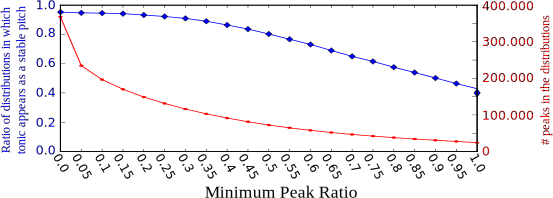
\includegraphics[width=.8\columnwidth]{figures/min_peak_ratio}
\caption{Total number of peaks and the ratio between the number of tonic hits and number of all distributions.}
\label{fig:min_peak_ratio}
\end{figure}

By inspecting Figure~\ref{fig:min_peak_ratio}, we observe that the probability of finding the tonic among the peaks is very high for minimum peak thresholds less than $0.4$ in the expense of an exponential increase in the tonic candidates (peaks) and hence in the processing time. Since our scenario can tolerate a moderate increase in processing time, we selected the minimum peak threshold as $0.15$.

Table 2 shows the best results obtained after grid search. For mode recognition, multi-distribution per mode model yields an accuracy of $71.8\%$ with the best parameter set while highest accuracy using single distribution per mode is $38.7\%$. For tonic identification multi-distribution per mode performs with accuracy above $95\%$ in $20$ parameter sets and above $90\%$ accuracy in $299$ parameter sets out of $1440$ experiments, where the highest accuracy obtained is $95.8\%$. Hence, the method is robust to a variety of parameter selections for tonic identification. On the other hand, Single distribution per mode model yields $89.8\%$ accuracy with the best parameter set. For joint estimation the multi-distribution per mode model performs with $63.6\%$ accuracy in the best configuration while single distribution yields $27.6\%$.

For all three considered tasks, the optimal choices for \textbf{P3}, \textbf{P5} and \textbf{M} turned out to be Bhattacharyya distance, PCD and multi-distribution per mode.
{\renewcommand{\arraystretch}{1.25}
\begin{table}[H]
\label{tab:best_results}
\caption{Best parameter sets for each task. For all tasks PCDs using Bhattacharyya distance and traning multiple distributions per mode gives the best results.}
 \begin{center}
%\begin{tabular}{ |l|l|l|l|l|l| }
\begin{tabular}{ l c c c c }
\hline
\textbf{Task} & \textbf{$\sigma$} & \textbf{$\beta$} & \textbf{k} & \textbf{Accuracy}\\ \hline
Tonic & 7.5 & 15 & 3 & \textbf{95.8\%}\\
 \hline
Mode & 25 & 25 & 10, 15 & \textbf{71.8\%} \\ \hline
Joint & 20 & 15 & 5 & \textbf{63.6\%}\\ \hline
\end{tabular}
\end{center}
\end{table}}

The method proposed in~\cite{sercan_tonic} is the state of the art for tonic identification in OTMM culture. We evaluated this approach on our dataset and obtained $79.9\%$ accuracy. Multi-distribution per mode method outperforms this method either if the mode is known ($95.8\%$ accuracy) or not ($91.5\%$ tonic accuracy in joint estimation) with the majority of sub-optimal parameter sets. The best tonic identification accuracy using PDs and single-distribution per mode is $49.8$. Figure~\ref{fig:tonic_distribution} shows the distribution of the octave-wrapped cent distance (Section~\ref{sec:experiment_setup}) between the estimated and the annotated tonic for each test and for all the parameter sets with $7.5$ cent bin size. 

\begin{figure}
\centering
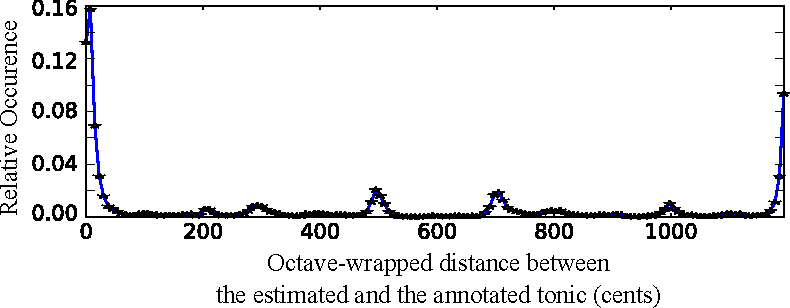
\includegraphics[width=.8\columnwidth]{figures/tonic_deviation_distribution}
\caption{The distribution of octave-wrapped distances between the estimated and annotated tonic for all parameter sets with $7.5$ cent bin size.}
\label{fig:tonic_distribution}
\end{figure}

These experiments revealed that certain parameter selections significantly improve or diminish the methods' performances. These observations are listed below as a guidance:

\begin{itemize}[noitemsep]
\item \textbf{M:} Multi-distribution training model performs significantly better than single-distribution training model.
\item \textbf{F2:} PCD significantly outperforms PD.
\item \textbf{P1:} Smaller bin size yields better results, however there is no significant distinction between $7.5$, $15$ and $25$ cent bin sizes. Note that these bin sizes significantly outperform 50 and 100 cent bin sizes.
\item \textbf{P2:} The $7.5$, $15$ and $25$ cent kernel widths significantly improves the accuracy of the models compared to $50$ and $100$ cent kernel widths. No smoothing performs slightly worse than $7.5$, $15$ and $25$ cent kernel widths. However, processing the distribution without smoothing is substantially slower due to the peak detection step.
\item \textbf{P3:} Using multi-distribution training model and PCDs, Bhattacharyya distance always yields the highest accuracy. It is significant except using $1-$intersection and $L1$ in tonic identification.
\item \textbf{P4:} Increasing the number of nearest neighbors of $k$ increases the accuracy. Nevertheless, the increase does not make a significant impact except $k = 1$, which performs significantly worse than higher $k$ values.
\item \textbf{P5:} In the tonic identification task, the true tonic is typically among the detected peaks for minimum peak ratios below $0.4$. Values smaller than $0.1$ increases the processing time without any meaningful improvement in tonic identification accuracy.
\end{itemize}

\section{Experiments on Hindustani and Carnatic Music}
\label{sec:hindustani_carnatic}

Recently, MORTY was used as a benchmark for raga/raag recognition of audio recordings of Hindustani and Carnatic music in comparison with two novel methods~\cite{gulati2016raga,gulati_network}. Below we explain the results briefly. Note that there already exists a method for tonic identification for these music traditions~\cite{sankalp_tonic}, which is reported to provide near perfect results. This method is used in both for the automatic tonic identification step. Therefore, the tonic identification and joint estimation using the methods in the toolbox are not applied during these experiments.

For the first of these methods~\cite{gulati2016raga}, the multi-distribution method was used as the state of the art of the culture. The methods are evaluated for $10$ raga and $40$ raga setups. The parameters are chosen as $\beta = 10$ cents, $\sigma = 10$ cents, $k = 1$ using Bhattacharyya distance. These experiments were conducted for both entire recordings and the $120$ seconds long excerpts. The full recording mode recognition yielded an accuracy of $89.5\%$, while the windowed excerpts yielded $82.2\%$ in the case of 10 raga scenario and $66.4\%$ and $74.1\%$ in the $40$ raga case, respectively.

In the latter work~\cite{gulati_network}, the proposed mode recognition method is applicable to both Hindustani and Carnatic traditions and the multi-distribution approach was again used as the state of the art for comparison. The used Carnatic dataset is composed of $40$ ragas and the Hindustani dataset $30$ ragas. The results for multi-distribution method was again only reported for the optimal parameter set, which is the same as the aforementioned work. This method performed $91.7\%$ accuracy on Hindustani and $73.1\%$ on Carnatic datasets.
%In the experiments we use the optimal parameters reported in~\cite{chordia}: We compute pitch class distributions with a bin size of $\beta=10$ cents. The kernel width $\sigma$ reported in~\cite{chordia} is in Hz scale, which would mean variable smoothing across octave. We empirically found $\sigma = 15$ cents as a reasonable value. We train multiple pitch class distributions per mode as described in~\cite{chordia}. In testing we use Bhattacharyya distance and select the nearest neighbor ($k = 1$). Note that there already exists a method for tonic identification for these music traditions~\cite{sankalp_tonic}, which is reported to provide near perfect results. We use this method for the automatic tonic identification instead of the methodology explained in Section~\ref{sec:training}. Below we explain the results briefly. Please refer to the respective papers~\cite{gulati_network,gulati2016raga} for further details.

%In~\cite{gulati_network} a method based on melodic contours is proposed for mode recognition. The method is compared against the methods proposed in~\cite{chordia} (multi-distribution) and~\cite{koduri2014intonation} on two datasets consisting Carnatic music recordings in 10 ragas and 40 ragas, respectively. The best accuracies obtained for the 10 raga dataset are $91.7\%$, $89.5\%$ and $70.01\%$ using the proposed method, MORTY and~\cite{koduri2014intonation}. Both the proposed methodology and MORTY obtained comparable results and they outperformed~\cite{koduri2014intonation}. In the 40 raga dataset our method ($74.1\%$ accuracy) outperformed both methods the proposed method ($69.6\%$ accuracy) and~\cite{koduri2014intonation} ($51.4\%$ accuracy).

%Later the same authors have proposed another feature for raga recognition~\cite{gulati2016raga}, which they term as ``time-delayed melody surface.'' The training and testing scheme is the same with the procedure explained in~\cite{chordia}. In the experiments The proposed feature was compared against pitch class distributions on a dataset of Hindustani recordings and the same dataset used in~\cite{gulati_network} with a different experimental setup. In both datasets the proposed feature ($97.7\%$ accuracy on Hindustani and $86.7\%$ accuracy on Carnatic dataset) has outperforms PCDs ($91.7\%$ accuracy on Hindustani and $73.1\%$ accuracy on Carnatic dataset).

\section{Discussion}\label{sec:discussion}

The drawback of the pitch distribution based methods is that they don't consider the temporal characteristics. When we inspected the results obtained from the experiments in~\ref{sec:experiments}, we observed that the confusions are mainly between makams, which either have very similar intervals in their scale or contain similar sets of pitches. Similarly in~\cite{gulati_network}, the proposed method was better in classifying phrase-based ragas, while our method was better at classifying scale based ones. The mode recognition using the feature proposed in~\cite{gulati2016raga} is able to capture both of these properties better with a slight increase in computational complexity.

In~\cite{sercan_tonic}, the authors showed that their method outperforms the tonic identification method in~\cite{bozkurt_tonic} (using PDs with single-model per mode) for OTMM. Our results validate the findings (the best is accuracy is $49.8$ as stated in Section~\ref{sec:results}). Nevertheless, we show that using PCDs with multi-model per mode is superior to both methods, even when the makam of the recording is not know and even if the makam is found erroneously in the joint estimation process. While the estimated tonic is typically around the annotation (Figure~\ref{fig:tonic_distribution}), the main confusion occurs around the fourth, fifth and seventh of the tonic, which typically act as the melodic centers and/or anchor points in the melodic progression~\cite{ozkan1984musiki}.

We suggest using multi-distribution models approach with Bhattacharyya distance and PCD. If the estimation accuracy is a top priority, we suggest choosing a small $\beta$, $\sigma$ ($7.5$ or $15$ cents) and minimum peak ratio $0.15$ as these parameters yield high accuracies. For use-cases like mobile or real-time applications where computational complexity plays a key role, $\beta$, $\sigma$ ($25$ cents) and minimum peak ratio ($0.4$) can be bigger, since reduced feature dimensions substantially decrease the computational complexity. The number of neighbors may be chosen as any value higher than $1$.

\section{Conclusion}\label{sec:conclusion}
We presented MORTY, an open toolbox for mode recognition and tonic identification. The toolbox generalizes the state-of-the-art in pitch distribution based classification for these tasks. It is designed with flexibility in mind such that it can be easily modified and optimized to analyse large audio corpora. We evaluated the implementation on the largest makam recognition dataset of Ottoman-Turkish makam music. Our generalized method outperformed the state-of-the-art methodologies proposed for mode recognition~\cite{bozkurt_makam} and tonic identification~\cite{bozkurt_tonic, atli2014makamFeature_atmm}. The toolbox has also been used to benchmark two novel mode recognition methodologies proposed for Indian art musics. 

MORTY is also used as a part of our makam music analysis toolbox.\footnote{\url{https://github.com/sertansenturk/tomato}} Currently it is used to analyze the tuning and obtain a statistical model for each note. We have analysed the whole audio collection of the CompMusic makam corpus~\cite{compmusic_corpus}. The automatic description obtained from the analysis is available via Dunya, CompMusic's prototype web-application for music discovery.\footnote{\url{http://dunya.compmusic.upf.edu/makam/}} In the future, we plan to apply dimension reduction and hashing techniques to summarize the features and speed up the classification for real-time mode and tonic estimation on short audio excerpts. We also hope that MORTY may be useful as a general tool for tonic identification, mode recognition and tuning analysis applied on different modal music traditions.

\section{Acknowledgements}This work is partly supported by the European Research Council under the European Unions Seventh Framework Program, as part of the CompMusic project (ERC grant agreement 267583)

\bibliographystyle{abbrv}
\bibliography{sigproc}

\end{document}
